% main.tex
\documentclass[a4paper,12pt]{article}

% ----------------------- Paquetes básicos ----------------------------------
\usepackage[utf8]{inputenc}
\usepackage[T1]{fontenc}
\usepackage[spanish]{babel}
\usepackage{graphicx}
\usepackage{subcaption}
\usepackage{caption}
\usepackage{listings}
\usepackage{amsmath}
\usepackage{amssymb}
\usepackage{float}
\usepackage{geometry}
\usepackage{fancyhdr}
\usepackage{enumitem}
\usepackage{booktabs}
\usepackage[hidelinks]{hyperref}
\usepackage{cleveref}
\usepackage{xcolor}

% ----------------------- Configuración global ------------------------------
\geometry{margin=2.5cm}
\graphicspath{{images/}}
\pagestyle{fancy}
\fancyhf{}
\lhead{Boot}
\rhead{TP Sistemas de Computación}
\cfoot{\thepage}

% ----------------------- Listings: lenguajes -------------------------------
\lstdefinelanguage{NASM}{
  morekeywords={section,global,extern,cli,sti,lgdt,lidt,add,and,or,jmp,call,
                mov,push,pop,ret,pusha,pushad,popa,popad},
  sensitive=true,
  morecomment=[l]{;},
  morestring=[b]',
}
\lstdefinelanguage{C}{
  morekeywords={EFI_STATUS,CHAR16,UINTN,UINT32,EFI_GUID,while,if,return,void,int},
  sensitive=true,
  morecomment=[l]{//},
  morecomment=[s]{/*}{*/},
  morestring=[b]',
}
\lstdefinelanguage{GDB}{
  morekeywords={target,remote,file,set,architecture,b,break,c,continue,
    si,stepi,info,registers,print,x,s,delete,layout,quit},
  sensitive=false,
  morecomment=[l]{\#},
}

% ----------------------- Listings: estilos ---------------------------------
\lstdefinestyle{NasmStyle}{
  language=NASM,
  basicstyle   =\ttfamily\small,
  numberstyle  =\tiny,
  numbers      =left,
  stepnumber   =1,
  frame        =single,
  captionpos   =b,
  keywordstyle =\color{blue},
  commentstyle =\itshape\color{gray!70},
  showstringspaces=false,
  extendedchars=true
}
\lstdefinestyle{CStyle}{
  language=C,
  basicstyle   =\ttfamily\small,
  numbers      =left,
  frame        =single,
  keywordstyle =\color{blue},
  commentstyle =\itshape\color{gray!70},
  showstringspaces=false
}
\lstdefinestyle{BashInputStyle}{
  language=Bash,
  basicstyle=\small\ttfamily,
  backgroundcolor=\color{lightgray!20},
  frame=single, framerule=0.4pt, framesep=3pt,
  xleftmargin=6pt, xrightmargin=6pt,
  breaklines=true,
  keywordstyle=\color{blue}\bfseries,
  commentstyle=\color{green!60!black},
  stringstyle=\color{purple},
  numbers=none,
  showstringspaces=false
}
\lstdefinestyle{GdbStyle}{
  language=GDB,
  basicstyle  =\small\ttfamily,
  backgroundcolor=\color{cyan!10},
  frame       =single, framerule=0.4pt, framesep=3pt,
  xleftmargin =6pt, xrightmargin=6pt,
  breaklines  =true,
  keywordstyle=\color{red!80!black}\bfseries,
  commentstyle=\color{green!60!black},
  stringstyle =\color{purple},
  numbers     =none,
  showstringspaces=false
}

% Estilo por defecto si olvidas 'style='
\lstset{
  basicstyle=\ttfamily\small,
  frame=single,
  captionpos=b
}

% ----------------------- Metadatos del documento ---------------------------
\title{\textbf{TP Sistemas de Computación}\\\large Práctico: UEFI / Bootloader en NASM}
\author{Alumno: Nombre Apellido \\ Materia: Sistemas de Computación \\ Comisión: XX}
\date{\today}

% ----------------------- Inicio del documento ------------------------------
\begin{document}

\begin{titlepage}
    \begin{center}
        {\LARGE \textbf{Universidad Nacional de Córdoba}}\\[1.5cm]

        
\includegraphics[scale=0.4]{images/logo2.png}\\[1.5cm]

        {\large Facultad de Ciencias Exactas, Físicas y Naturales}\\
        {\large Escuela de Electrónica y Computacion}\\[1cm]

        \rule{\linewidth}{0.5mm}\\[0.4cm]
        {\Large \textbf{Cátedra de Sistemas de Computacion}}\\[0.3cm]
        {\LARGE \textbf{Trabajo de Laboratorio 3}}\\[0.3cm]

        \rule{\linewidth}{0.5mm}\\[1cm]

        \begin{flushleft}
        {\large 
            \textbf{Profesor Titular:} Ing. Javier Alejandro JORGE\\
            \textbf{Profesor Adjunto:} -\\[0.5cm]
            \textbf{Integrantes:}\\
            Trucchi, Genaro\\
            Trachtta, Agustin\\
            Rodriguez, Mateo\\
        }
        \end{flushleft}

        \vfill

        {\large \today}
    \end{center}
\end{titlepage}


\tableofcontents
\clearpage

\section{¿Qué es un módulo del kernel y para qué se usa?}

Un \textbf{módulo del kernel} es un fragmento de código que puede ser cargado o descargado en el kernel de~Linux según sea necesario, extendiendo la funcionalidad del sistema operativo sin necesidad de recompilar o reiniciar el sistema. En esencia, los módulos permiten tener un kernel modular y flexible: podemos agregar o quitar características del kernel en tiempo de ejecución.

\subsection*{Algunos usos típicos de los módulos del kernel son}
\begin{itemize}
  \item \textbf{Controladores de dispositivos (drivers)}: permiten al kernel comunicarse con hardware específico (ej.\ controladores de gráficos, Wi-Fi, dispositivos de audio, etc.). De hecho, muchos controladores de hardware se implementan como módulos cargables.
  \item \textbf{Sistemas de archivos}: el soporte para nuevos tipos de sistemas de archivos puede añadirse como módulo.
  \item \textbf{Extensiones del núcleo}: cualquier funcionalidad adicional (monitorizar temperaturas, agregar funcionalidades de seguridad, etc.) puede implementarse como módulo cargable.
  \item \textbf{Módulos privativos o de terceros}: por ejemplo, controladores propietarios (como el driver NVIDIA) que no están incluidos en el kernel base se distribuyen como módulos separados.
\end{itemize}

Sin módulos, tendríamos que compilar todas estas funcionalidades directamente en el kernel monolítico, haciendo el núcleo más grande y obligando a reconstruir y reiniciar el sistema cada vez que quisiéramos una nueva funcionalidad. Gracias a los módulos, el kernel puede mantenerse ligero y ampliable dinámicamente.

\subsection*{Módulos \emph{vs.} programas en espacio de usuario}
A diferencia de una aplicación de usuario normal (un programa común que ejecutamos en Linux), un módulo del kernel corre en modo privilegiado dentro del núcleo. Los programas de usuario se ejecutan en el \emph{espacio de usuario} y deben llamar a servicios del sistema operativo (mediante llamadas al sistema) para realizar acciones privilegiadas. En cambio, un módulo forma parte del kernel: tiene acceso directo al hardware y a las estructuras internas del sistema, con las ventajas y riesgos que esto implica (ver sección~\ref{sec:compilacion}). Además, un programa de usuario es un ejecutable con un punto de entrada (\lstinline!main()! típicamente), mientras que un módulo es esencialmente un fichero objeto especial (\texttt{.ko}) que se inserta en el kernel y no tiene \lstinline!main()! propio. Más adelante profundizaremos en estas diferencias de estructura y contexto de ejecución.

\section{Estructura de un módulo de kernel (\texttt{module\_init}, \texttt{module\_exit}, Makefile)}

Para crear un módulo de kernel simple, debemos seguir una estructura específica ya que, como mencionamos, no existe la función \lstinline!main()! en un módulo. En su lugar, un módulo define dos funciones especiales registradas mediante macros proporcionadas por el kernel:

\begin{itemize}
  \item \textbf{Función de inicialización (\texttt{module\_init})}: es la función que se ejecuta cuando el módulo se inserta (carga) en el kernel. Se registra con la macro \texttt{module\_init(nombre\_función\_init)}. En esta rutina se realiza la configuración necesaria: por ejemplo, registrar manejadores, inicializar estructuras de datos, imprimir un mensaje de log, etc. Al insertarse el módulo, el kernel llamará automáticamente a esta función.
  \item \textbf{Función de salida (\texttt{module\_exit})}: es la función ejecutada al remover el módulo del kernel. Se registra con la macro \texttt{module\_exit(nombre\_función\_exit)}. En esta rutina se liberan recursos, se anulan registros realizados en la \texttt{init} y, en general, se realiza cualquier limpieza necesaria antes de que el módulo sea descargado.
\end{itemize}

Estas dos funciones actúan, en cierta forma, como el ``constructor'' y ``destructor'' del módulo. Los módulos deben tener una función de entrada y otra de salida definidas de esta forma. Un código mínimo de un módulo podría ser:

\begin{lstlisting}[language=C]
#include <linux/module.h>
#include <linux/init.h>

static int __init mi_modulo_init(void) {
    printk(KERN_INFO "Mi modulo ha sido insertado!\n");
    return 0; /* 0 indica carga exitosa */
}

static void __exit mi_modulo_exit(void) {
    printk(KERN_INFO "Mi modulo ha sido removido.\n");
}

module_init(mi_modulo_init);
module_exit(mi_modulo_exit);

MODULE_LICENSE("GPL");
MODULE_AUTHOR("Tu Nombre");
MODULE_DESCRIPTION("Modulo de ejemplo Hola Mundo");
\end{lstlisting}

Ademas del codigo C del modulo, es crucial proveer un \textbf{Makefile} adecuado para compilar el modulo contra el kernel. Los modulos se compilan utilizando el sistema de construccion del kernel (\emph{Kbuild}). Un Makefile tipico para un modulo simple podria contener:

\begin{lstlisting}[language=make]
obj-m := mimodulo.o

KDIR := /lib/modules/$(shell uname -r)/build
PWD  := $(shell pwd)

all:
	$(MAKE) -C $(KDIR) M=$(PWD) modules

clean:
	$(MAKE) -C $(KDIR) M=$(PWD) clean
\end{lstlisting}

Este Makefile indica que queremos construir un objeto modular \texttt{mimodulo.ko} a partir de \texttt{mimodulo.c}. Usamos la regla especial \texttt{obj-m} para listar el nombre del modulo. Luego invocamos \texttt{make -C /lib/modules/\$(uname -r)/build M=\$(PWD)} para que el sistema de compilacion del kernel compile nuestro codigo como modulo externo. Esto requiere tener instalados los \emph{headers} o el codigo fuente del kernel correspondiente a nuestra version (en Debian/Ubuntu, instalar el paquete \texttt{linux-headers-\$(uname -r)}).

Una vez escrito el código fuente y el Makefile, el flujo es: compilar con \texttt{make} para obtener el archivo \texttt{mimodulo.ko}, y luego podremos insertarlo en el kernel con herramientas como \texttt{insmod} (ver sección~\ref{sec:compilacion}).

\section{Compilación e instalación de módulos (\texttt{make}, \texttt{insmod}, \texttt{rmmod}, \texttt{lsmod}, \texttt{modinfo})}
\label{sec:compilacion}

\subsection*{Compilación}
Tras preparar el código fuente del módulo y su Makefile, la compilación se realiza normalmente con el comando \texttt{make}. Esto genera un archivo objeto con extensión \texttt{.ko} (\emph{kernel object}). Por ejemplo, siguiendo el Makefile antes mencionado, simplemente ejecutar \texttt{make} en el directorio del código producirá \texttt{mimodulo.ko}. Si es necesario limpiar archivos de compilación previos, \texttt{make clean} ayudará.

\subsection*{Inserción de un módulo (\texttt{insmod}/\texttt{modprobe})}
Para instalar un módulo en el kernel en ejecución, se utiliza la utilidad \texttt{insmod}. Por ejemplo:
\begin{lstlisting}
sudo insmod mimodulo.ko
\end{lstlisting}
\texttt{insmod} inserta el modulo especificado directamente, pero no resuelve dependencias automaticamente. Si el modulo requiere de otros modulos (por ejemplo, un driver puede depender de otro modulo \emph{core}), esas dependencias deben estar cargadas previamente. Alternativamente, se puede usar \texttt{modprobe}, que si resuelve dependencias consultando la base de datos de modulos del sistema. \texttt{modprobe mimodulo} buscaria \texttt{mimodulo.ko} en las rutas de modulos instalados del sistema (normalmente en \texttt{/lib/modules/\$(uname -r)/\dots}) e intentaria cargarlo junto con cualquier dependencia declarada.

\subsection*{Verificación de carga (\texttt{lsmod}, \texttt{/proc/modules}, \texttt{dmesg})}
Después de insertar un módulo, es útil comprobar que esté efectivamente cargado y revisar mensajes de log:
\begin{itemize}
  \item El comando \texttt{lsmod} lista todos los módulos actualmente cargados en el kernel. Si nuestro módulo se cargó correctamente, \texttt{lsmod | grep mimodulo} debería mostrarlo, indicando también su tamaño y el número de referencias (usos) que tiene. Internamente, \texttt{lsmod} simplemente formatea la información disponible en el archivo virtual \texttt{/proc/modules}. Podemos inspeccionar directamente \texttt{/proc/modules} para ver información similar en formato texto.
  \item El comando \texttt{dmesg} muestra el registro de mensajes del kernel (el \emph{kernel ring buffer}). Nuestro módulo, al cargar, probablemente imprimió algo con \texttt{printk()}. Usando \texttt{dmesg | tail} veremos los últimos mensajes del kernel, donde debería aparecer el mensaje de inicialización del módulo (ej.\ ``Mi módulo ha sido insertado!''). Esto confirma que la función \texttt{module\_init} se ejecutó. Igualmente, al remover, habrá mensajes de salida del módulo.
\end{itemize}

\subsection*{Remoción de un módulo (\texttt{rmmod})}
Para quitar un módulo del kernel, se utiliza \texttt{rmmod}. Ejemplo:
\begin{lstlisting}
sudo rmmod mimodulo
\end{lstlisting}
Esto invoca la rutina de limpieza (\texttt{module\_exit}) del módulo y luego descarga el código del kernel. Tras hacer \texttt{rmmod}, conviene nuevamente chequear \texttt{lsmod} (para confirmar que ya no figura) y \texttt{dmesg} (debería mostrar el mensaje de que el módulo se removió correctamente).

\subsection*{Información de un módulo (\texttt{modinfo})}
La herramienta \texttt{modinfo} muestra metadatos y detalles de un módulo compilado. Por ejemplo,
\begin{lstlisting}
modinfo mimodulo.ko
\end{lstlisting}
listará información como: descripción, autor, licencia, alias, versión de \emph{vermagic} (la versión de kernel para la que fue compilado) y si está firmado digitalmente (más sobre firma en la siguiente sección). Esto es útil para inspeccionar rápidamente las propiedades de un módulo antes de cargarlo o para verificar si la compilación se hizo para la versión correcta del kernel.

\subsection*{Ejemplo práctico resumido}
Supongamos que ya compilamos \texttt{mimodulo.ko} exitosamente:
\begin{enumerate}
  \item Insertamos el módulo:\newline
    \texttt{sudo insmod mimodulo.ko}
  \item Verificamos con \texttt{lsmod} – deberíamos ver \texttt{mimodulo} en la lista de módulos cargados. También podríamos hacer:\newline
    \texttt{cat /proc/modules | grep mimodulo}
  \item Miramos el log:\newline
    \texttt{dmesg | tail -n 5}\newline
    y vemos algo como ``Mi módulo ha sido insertado!'' indicando que la \texttt{init} corrió.
  \item Probamos quitarlo:\newline
    \texttt{sudo rmmod mimodulo}
  \item Nuevamente \texttt{dmesg | tail} mostrará ``Mi módulo ha sido removido.'' de la función \texttt{exit}, y \texttt{lsmod} confirmará que ya no está en memoria.
  \item Ejecutamos \texttt{modinfo mimodulo.ko} para ver los metadatos: por ejemplo, confirmamos que la licencia es GPL (lo cual es importante; si un módulo no está marcado GPL, el kernel lo registra como ``\emph{proprietary}'' y ciertas funciones internas podrían no estar disponibles para ese módulo).
\end{enumerate}

Esta secuencia básica permite compilar un módulo fuera del árbol del kernel, insertarlo, verificar su funcionamiento y luego retirarlo de manera limpia.

\section{Seguridad: firma de modulos para Secure Boot (por que es importante y como se realiza?)}

Cuando Secure Boot (arranque seguro UEFI) esta habilitado en un sistema, el firmware y el cargador de arranque solo permitiran arrancar codigo firmado con claves de confianza. Esta cadena de confianza se extiende hasta el propio kernel y sus modulos: no basta con que el kernel este firmado, los modulos del kernel tambien deben estar firmados digitalmente para que el kernel los cargue bajo Secure Boot. El objetivo es prevenir que codigo no autorizado o malicioso (como un rootkit) se inyecte en el kernel.

\subsection*{Por que es importante?}

Sin firma obligatoria, un atacante con privilegios de superusuario podria cargar un modulo malicioso que comprometa el sistema a nivel de kernel (por ejemplo, ocultar procesos, capturar contrasenas, etc.). La firma de modulos garantiza que solo modulos con una firma valida—es decir, provenientes de una fuente confiable—puedan insertarse cuando Secure Boot esta activo, reforzando la seguridad del sistema. Una recomendacion frecuente de seguridad del kernel es evitar cargar modulos no firmados para dificultar la instalacion de rootkits.

\subsection*{Como funciona la verificacion?}

Al compilar el kernel, las distribuciones incluyen una clave privada con la que firman todos sus modulos oficiales; el kernel incorpora (o tiene acceso a) la correspondiente clave publica. Cuando Secure Boot esta activo, el kernel comprueba la firma de cada modulo cargado contra las claves X.509 de confianza que posee en sus llaveros internos (\texttt{.builtin\_trusted\_keys} y \texttt{.platform}). En terminos simples: el modulo lleva una firma digital anexada y el kernel solo lo aceptara si puede verificar esa firma con alguna clave publica reconocida como confiable. Si la firma no es valida o el modulo no esta firmado, la carga falla.

La documentacion de Red Hat indica que con Secure Boot activo (o con la opcion \texttt{module.sig\_enforce} habilitada) ``solo se pueden cargar modulos del kernel firmados cuyas firmas se hayan autenticado contra claves del llavero de confianza del sistema (\texttt{.builtin\_trusted\_keys}) o de la plataforma (\texttt{.platform}); ademas la clave publica del firmante no debe estar revocada (\texttt{.blacklist})''. En cambio, si Secure Boot esta deshabilitado, el kernel permite cargar modulos no firmados libremente (o modulos firmados cuya clave no conozca), es decir, la verificacion de firmas deja de ser obligatoria.

\subsection*{Como se firma un modulo?}

El proceso general para firmar un modulo personalizado es:

\begin{enumerate}
  \item \textbf{Generar un par de claves X.509 (privada y publica).} Puede ser una clave autofirmada. Por ejemplo, con \texttt{openssl} se crea una clave RSA y un certificado X.509, indicando en el campo \emph{Common Name} algo como ``Module Signing Key''.
  \item \textbf{Firmar el modulo \texttt{.ko}.} El kernel provee \texttt{scripts/sign-file}, que aplica una firma PKCS\#7 al modulo usando la clave privada. Ejemplo:  
  \texttt{scripts/sign-file sha256 clave\_privada.pem certificado\_publico.pem mimodulo.ko}  
  Esto calcula un hash SHA-256 del modulo y lo firma; \texttt{modinfo mimodulo.ko} mostrara campos como \texttt{sig\_id}, \texttt{sig\_key}, \texttt{sig\_hashalgo}.
  \item \textbf{Registrar la clave publica en el sistema.} En entornos con Secure Boot se suele usar MOK (Machine Owner Key). Se convierte el certificado a DER y se ejecuta  
  \texttt{sudo mokutil --import cert.der}  
  Tras reiniciar y confirmar en la interfaz UEFI, la clave quedara en el llavero \texttt{.platform} o en el llavero de sistema, y el kernel la reconocera.
\end{enumerate}

Una vez registrada la clave, \texttt{insmod mimodulo.ko} funcionara sin error; si la clave no estuviera registrada, apareceria ``Required key not available'' y el modulo no se cargaria.

\section{Diferencia entre espacio de usuario y espacio de kernel (seguridad e implicancias de errores como segmentation fault)}

Los sistemas operativos modernos dividen la ejecucion en dos espacios de memoria bien diferenciados: \emph{espacio de usuario} y \emph{espacio de kernel}.

\subsection*{Espacio de usuario (user space)}

\begin{itemize}
  \item Aloja las aplicaciones normales con privilegios limitados.
  \item Cada proceso tiene su propio espacio de direcciones virtuales y no puede acceder directamente a la memoria del kernel ni a la de otros procesos.
  \item Si un programa intenta leer o escribir fuera de su rango permitido, el hardware y el kernel lo impiden, provocando un \textit{segmentation fault}.
  \item Un fallo en una aplicacion de usuario rara vez compromete todo el sistema: se termina solo ese proceso.
\end{itemize}

\subsection*{Espacio de kernel}

\begin{itemize}
  \item Reservado para el nucleo y sus extensiones (drivers, modulos cargados).
  \item Corre en modo privilegiado (ring 0 en x86), con acceso completo al hardware y a toda la memoria.
  \item Un error aqui (por ejemplo, desreferenciar un puntero invalido) puede causar un \textit{oops} del kernel o un \textit{kernel panic}, bloqueando por completo el sistema.
  \item No existen las mismas barreras de aislamiento que en user space; por eso los modulos deben ser confiables.
\end{itemize}

\subsection*{Implicancias de seguridad}

La separacion usuario/kernel existe para que el kernel actue de guardian: un programa malicioso en user space esta confinado; si intenta algo prohibido el kernel lo detiene. En cambio, ejecutar codigo en kernel space (mediante un modulo malicioso o explotando un bug en un driver) otorga control total: se pueden desactivar protecciones, ocultar procesos, espiar datos de cualquier aplicacion, etc. De ahi la importancia de cargar solo modulos de confianza.

\subsection*{Segmentation fault vs. errores en kernel}

\begin{itemize}
  \item \textbf{User space:} un \textit{segmentation fault} ocurre al acceder memoria invalida; el kernel mata el proceso y libera recursos, manteniendo el sistema estable. Herramientas como \texttt{gdb} y \emph{core dumps} facilitan la depuracion.
  \item \textbf{Kernel space:} un acceso invalido genera un \textit{oops}; si es grave, un \textit{kernel panic}. No hay entorno aislado: todo el sistema puede caer. Depurar implica revisar trazas del kernel o usar herramientas como \texttt{kgdb}.
\end{itemize}

\section{Llamadas al sistema con \texttt{strace} y diferencia con las funciones disponibles en el kernel}

Una llamada al sistema (\emph{system call}) es el mecanismo mediante el cual un programa en espacio de usuario solicita un servicio al kernel (por ejemplo, ``lee este archivo'', ``envia estos datos por la red'', etc.). Se puede pensar en las \emph{syscalls} como la frontera de comunicacion entre \emph{user space} y \emph{kernel space}.  
La herramienta \texttt{strace} resulta sumamente util para observar en tiempo real que llamadas al sistema hace un programa de usuario; basicamente traza esa ``capa fina'' de interaccion entre un proceso y el kernel.

Por ejemplo, si escribimos un programa en~C que hace \texttt{printf("Hola mundo\textbackslash n")} y lo ejecutamos, internamente ese \texttt{printf} terminara invocando la llamada al sistema \texttt{write()} para enviar texto a la salida estandar (descriptor~1). Si corremos \texttt{strace ./programa}, veremos una traza de todas las \emph{syscalls} realizadas por el proceso: aparecera una linea con \texttt{write(1, "Hola mundo\textbackslash n", 11)} y su valor de retorno, ademas de otras llamadas como \texttt{brk} (ajuste de \emph{heap}), \texttt{exit} al terminar, etc. \texttt{strace} intercepta estas llamadas mediante la funcionalidad \texttt{ptrace} del kernel y las imprime para nuestro analisis. Tambien podemos usar \texttt{strace -c} para un resumen estadistico (cuentas y tiempo), o \texttt{strace -tt} para marcas de tiempo, entre otras opciones.

Esto evidencia que un programa en \emph{user space} no accede al hardware ni realiza funciones privilegiadas por si mismo, sino que todo lo ejecuta pidiendoselo al kernel mediante \emph{syscalls}. La libreria de~C (\texttt{glibc}) provee funciones de mas alto nivel (\texttt{printf}, \texttt{open}, \texttt{socket}, etc.), pero casi todas terminan en una llamada al sistema subyacente (\texttt{write}, \texttt{openat}, \texttt{socket}, ...). De esta forma, las operaciones disponibles para un programa de usuario son esencialmente las que brinda la API del sistema operativo via llamadas al sistema (junto con las funciones de biblioteca que las envuelven). Podemos listar todas las \emph{syscalls} consultando \texttt{man~2 syscalls}: Linux define cientos de llamadas, pero siguen siendo un conjunto limitado y bien especificado de servicios que el kernel expone.

En contraste, un modulo de kernel no realiza llamadas al sistema (no tendria sentido: ya se ejecuta dentro del kernel). En su lugar, un modulo puede invocar directamente cualquier funcion exportada por el kernel. El conjunto de funciones disponibles es enorme: basicamente todas las declaradas con \texttt{EXPORT\_SYMBOL}, \texttt{EXPORT\_SYMBOL\_GPL}, etc. Por ejemplo, un modulo puede llamar a \texttt{printk()} para imprimir logs, usar \texttt{kmalloc} para asignacion de memoria en kernel, registrar dispositivos, etc. No puede usar funciones de \texttt{glibc} u otras librerias de usuario (\texttt{printf}, \texttt{malloc}, ...); en su lugar existen equivalentes del kernel.

Si un modulo intenta invocar una funcion que el kernel no haya exportado, la carga fallara con ``simbolo desconocido''. Ademas, no existe una herramienta equivalente a \texttt{strace} para modulos, porque no hay \emph{syscalls} involucradas una vez dentro del kernel. Para analizar un modulo se recurre a depuracion del kernel, revisando \texttt{/proc/kallsyms} (tabla de simbolos) o instrumentando el codigo con \texttt{printk}. \texttt{/proc/kallsyms} muestra direcciones de funciones y variables exportadas—requiere normalmente permisos de \texttt{root} y, segun configuracion, puede ocultar direcciones exactas.

\section{Archivos y directorios relevantes: \texttt{/proc}, \texttt{/dev}, \texttt{/lib/modules/\$(uname -r)/kernel}}

Linux expone informacion sobre el kernel, los procesos y el hardware mediante sistemas de archivos virtuales y directorios especificos. Los mas importantes al trabajar con modulos y drivers son \texttt{/proc}, \texttt{/dev} y el arbol de modulos instalados en \texttt{/lib/modules}.

\subsection*{\texttt{/proc}}

Es un sistema de archivos virtual (no existe en disco) montado en \texttt{/proc}. Contiene una vista en forma de archivos de muchos aspectos del estado del kernel, generada dinamicamente. Archivos clave:

\begin{itemize}
  \item \texttt{/proc/modules}: lista los modulos actualmente cargados (nombre, tamano, cuenta de usos). Equivale a la salida de \texttt{lsmod}. Se actualiza al cargar o descargar modulos.
  \item \texttt{/proc/kallsyms}: tabla de simbolos del kernel (funciones y variables exportadas). Una vez cargado un modulo, sus simbolos exportados aparecen aqui. Por seguridad, algunos kernels restringen la visibilidad de direcciones a usuarios no privilegiados.
  \item Otros archivos como \texttt{/proc/cpuinfo}, \texttt{/proc/iomem}, \texttt{/proc/interrupts} proveen detalles de hardware, utiles para diagnosticar que recursos manejan ciertos drivers.
\end{itemize}

\subsection*{\texttt{/dev}}

Contiene los nodos de dispositivo (\emph{device nodes}) que representan perifericos manejados por drivers. Al cargar un modulo que implementa un driver de caracter o bloque, este registra un mayor/menor y usualmente udev crea una entrada en \texttt{/dev}. Por ejemplo, al insertar el driver de una camara web puede aparecer \texttt{/dev/video0}. Los programas de usuario interactuan con el driver leyendo o escribiendo en ese nodo. No todos los modulos crean nodos en \texttt{/dev}; un modulo de sistema de archivos o uno de \emph{netfilter} no requiere hacerlo.

\subsection*{Directorio de modulos instalados}

Los modulos compilados para una version determinada del kernel se almacenan en
\texttt{/lib/modules/<version>/kernel/}. Por ejemplo, para un kernel \texttt{5.15.0-50-generic} existe:

\begin{center}
\texttt{/lib/modules/5.15.0-50-generic/kernel/}
\end{center}

Alli hay subdirectorios por categoria (drivers de sonido, red, FS, etc.) con archivos \texttt{.ko}. Este es el repositorio que \texttt{modprobe} consulta.

\begin{itemize}
  \item \texttt{ls -R /lib/modules/\$(uname -r)/kernel}: lista recursivamente todos los modulos disponibles para el kernel actual.
  \item Archivos como \texttt{modules.dep} indican dependencias entre modulos (generados por \texttt{depmod}).
  \item Algunas distribuciones mantienen \texttt{modules.sign} o \texttt{modules.sig} con hashes o firmas de los modulos oficiales.
\end{itemize}

\subsection*{Herramientas de consulta}

\begin{itemize}
  \item \texttt{lsmod}: muestra modulos cargados (lee \texttt{/proc/modules}).
  \item \texttt{modinfo <modulo>}: consulta metadatos del modulo ubicado en \texttt{/lib/modules/<ver>} sin requerir ruta completa.
  \item \texttt{lspci -k}: indica para cada dispositivo PCI que driver (modulo) esta en uso y que otros podrian manejarlo.
\end{itemize}

En conjunto, \texttt{/proc}, \texttt{/dev} y \texttt{/lib/modules} permiten observar el estado del kernel y gestionar modulos. Por ejemplo, si \texttt{insmod} falla, se revisa \texttt{dmesg}; si \texttt{modprobe} no encuentra un modulo, se comprueba que exista en \texttt{/lib/modules} y se ejecuta \texttt{depmod}. Conocer estas rutas y archivos es esencial para diagnostico y desarrollo de drivers.

\section{Drivers y deteccion de hardware (\texttt{hwinfo}, \texttt{lspci}, \texttt{lsusb}, etc.)}

Los drivers de hardware en Linux suelen ser modulos del kernel que se encargan de controlar un dispositivo fisico especifico o una familia de dispositivos. Para saber que hardware tenemos y que modulo (driver) lo maneja, disponemos de varias herramientas:

\begin{itemize}
  \item \texttt{lspci}: Lista los dispositivos PCI/PCIe del sistema (tarjetas graficas, controladoras SATA, tarjetas de red, etc. en el bus~PCI). Use \texttt{-v} (verbose) o \texttt{-vv} para mas detalle. De especial utilidad es \texttt{lspci -k}, que muestra, para cada dispositivo~PCI, que \emph{kernel driver} esta usando y que \emph{kernel modules} estan disponibles para ese dispositivo.

\vspace{0.3em}
Ejemplos:
\begin{lstlisting}
$ lspci -v -s 02:00.0     # informacion detallada de un dispositivo especifico
$ lspci -nn -k | grep -A3 Network
\end{lstlisting}

En la salida veremos lineas como: \texttt{Kernel driver in use: e1000e} y \texttt{Kernel modules: e1000e}, indicando que el dispositivo (p. ej. una tarjeta de red Intel) esta siendo manejado por el driver \texttt{e1000e}. Si hubiera modulos alternativos compatibles, aparecerian listados despues de \texttt{Kernel modules}. Para una GPU~NVIDIA, podria verse \texttt{Kernel driver in use: nvidia} y \texttt{Kernel modules: nvidia, nouveau}. \texttt{lspci -k} agrega dos lineas clave segun documentacion de Red~Hat: \texttt{Kernel driver in use} y \texttt{Kernel modules}.
  \item \texttt{lsusb}: Similar a \texttt{lspci} pero para dispositivos USB. Lista los dispositivos conectados al bus~USB. No indica directamente el modulo, pero sabemos que muchos dispositivos USB (almacenamiento, camaras, etc.) son manejados por subsistemas como \texttt{usb-storage}, \texttt{uvcvideo}, etc. Se puede correlacionar con \texttt{dmesg} al conectar el dispositivo o revisando \texttt{/sys/bus/usb/devices}.
  \item \texttt{hwinfo}: Herramienta exhaustiva (comun en OpenSUSE, disponible en otras distros) que provee informacion detallada del hardware. \texttt{hwinfo --short} da un resumen y \texttt{hwinfo --all} da detalles, incluyendo que driver esta asociado a cada dispositivo. Instalable en Debian/Ubuntu con \texttt{sudo apt install hwinfo}.
  \item Otros: \texttt{lshw} (lista hardware en jerarquia y puede mostrar drivers), \texttt{inxi -Fxxx} (info general del sistema), \texttt{dmidecode} (info BIOS/UEFI), y archivos en \texttt{/sys} como \texttt{/sys/bus/pci/devices/...} que exponen relaciones dispositivo--modulo.
\end{itemize}

\paragraph{Deteccion de hardware y modulos cargados.}  
Una practica comun es comparar la lista de modulos cargados (\texttt{lsmod}) entre diferentes sistemas para ver diferencias debidas al hardware. Por ejemplo, un equipo con GPU~Intel tendra \texttt{i915}, otro con NVIDIA tendra \texttt{nvidia} o \texttt{nouveau}, otro con AMD tendra \texttt{amdgpu}. Tambien se puede listar ``modulos disponibles pero no cargados'': p. ej. \texttt{pcspkr} puede existir en \texttt{/lib/modules} pero estar en blacklist. Estas comparaciones ayudan a mapear hardware $\leftrightarrow$ modulo.

En Linux moderno, \emph{udev} y el kernel auto-cargan modulos al detectar hardware: al conectar un USB, el kernel emite un \emph{uevent} y \emph{udev} carga el driver adecuado si esta disponible. Si un dispositivo no funciona, se puede buscar su ID con \texttt{lspci -nn} o \texttt{lsusb -v} y averiguar que modulo lo soporta.

Resumen: con estas herramientas mapeamos hardware y modulos, diagnostico esencial: \emph{``¿por que no funciona el WiFi?''} \textrightarrow{} revisamos \texttt{lspci -k}; si el driver no esta en uso, sabemos que modulo falta o no se cargo.

\section{Caso de estudio: Secure Boot, GRUB y el parche de Microsoft (Analisis del articulo de Ars Technica)}

Como aplicacion de los conceptos de modulos, firmas y Secure Boot, analicemos un incidente real mencionado en un articulo de Ars Technica: un parche de Microsoft relacionado con Secure Boot causo problemas en sistemas Linux dual-boot a mediados de 2024.

\subsection*{Contexto}

Existia una vulnerabilidad en GRUB2 (``BootHole'', 2020) que permitia sortear Secure Boot. Microsoft, que gestiona la base de datos de firmas UEFI (via Windows Update), preparo un parche para revocar componentes vulnerables. Tras dos anios de pruebas, el parche se lanzo en agosto de~2024. Se esperaba que solo afectara a sistemas Windows-only, pero impacto a equipos con dual-boot.

\subsection*{Sintoma}

Despues de instalar la actualizacion, muchos usuarios no pudieron arrancar Linux con Secure Boot habilitado. Aparecio el mensaje:

\begin{quote}\small
Verifying shim SBAT data failed: Security Policy Violation.\\
Something has gone seriously wrong: SBAT self-check failed: Security Policy Violation.
\end{quote}

Esto indica que \emph{shim} (bootloader firmado que carga GRUB) se bloqueo a si mismo al quedar en la lista de revocacion~SBAT incluida por Microsoft.

\subsection*{Consecuencia}

Los sistemas no podian iniciar Linux (ni siquiera GRUB); algunos quedaban solo con Windows. La solucion inmediata fue deshabilitar Secure Boot en el firmware UEFI. Alternativa mas tecnica: actualizar shim/GRUB a una version no revocada. Microsoft detuvo temporalmente la propagacion del parche en ciertos equipos tras reportes.

\subsection*{Lecciones}

\begin{itemize}
  \item La cadena de confianza de Secure Boot llega hasta shim/GRUB: si se revoca, el SO no carga.
  \item Los modulos del kernel firmados tambien estan sujetos a revocacion; un modulo critico con firma revocada seria rechazado.
  \item Mantener actualizados los componentes de arranque de Linux en dual-boot es vital para evitar bloqueos tras actualizaciones de seguridad.
  \item El rol de Microsoft como autoridad de firmas Secure Boot puede impactar a Linux; requiere coordinacion con las distribuciones.
\end{itemize}

Este caso demuestra como un cambio en las reglas de confianza (revocar un certificado) puede impedir cargar un SO, similar a lo que ocurre si intentamos cargar un modulo no firmado o con firma desconocida: el kernel lo rechazara por ``violacion de politica de seguridad''. Comprender estos mecanismos es esencial al desarrollar o instalar modulos en sistemas con Secure Boot.

\newpage
\section{Que es \texttt{checkinstall} y para que sirve?}

\texttt{checkinstall} es una utilidad que reemplaza temporalmente a la invocacion tradicional de \texttt{make install}.  
Su proposito principal es \textbf{generar un paquete binario} (DEB, RPM o TGZ, segun la distribucion) a partir de la instalacion que normalmente realizaria un script \texttt{Makefile}.  
En lugar de copiar archivos directamente al sistema de archivos, \texttt{checkinstall} intercepta el proceso, registra todos los archivos instalados y crea un paquete nativo:

\begin{itemize}[nosep]
  \item \textbf{Trazabilidad:} mantiene un registro exacto de los archivos instalados, lo que permite una desinstalacion limpia mediante el gestor de paquetes.
  \item \textbf{Consistencia:} integra el software compilado manualmente dentro de la base de datos de paquetes de la distribucion, evitando conflictos y archivos ``huerfanos''.
  \item \textbf{Portabilidad:} facilita distribuir el paquete a otros equipos con la misma distribucion sin recompilar.
\end{itemize}

\bigskip
Flujo simplificado de uso:

\begin{enumerate}[label=\arabic*.]
  \item \texttt{./configure \&\& make} \hfill (compila el proyecto)
  \item \texttt{sudo checkinstall --pkgname=mi-paquete --pkgversion=1.0} \hfill (intercepta \texttt{make install} y crea el .deb/.rpm)
  \item El paquete resultante aparece, por ejemplo, como \texttt{mi-paquete\_1.0-1\_amd64.deb}
  \item Instalacion normal con \texttt{sudo dpkg -i mi-paquete\_1.0-1\_amd64.deb}
\end{enumerate}

\newpage

%---------------------------------------------------------
\section{Empaquetar un ``Hello World'' con \texttt{checkinstall}}

A continuacion se muestra un ejemplo paso a paso para empaquetar un programa \emph{hello world} en~C:

\subsection*{1. Codigo fuente}

\begin{lstlisting}[language=C, caption={Archivo \texttt{hello.c}}]
#include <stdio.h>

int main(void) {
    puts("Hello World!");
    return 0;
}
\end{lstlisting}

\subsection*{2. Makefile minimal}

\begin{lstlisting}[language=make, caption={Archivo \texttt{Makefile}}]
CC  := gcc
CFLAGS := -Wall -O2
TARGET := hello

all:
	$(CC) $(CFLAGS) hello.c -o $(TARGET)

install:
	install -Dm755 hello /usr/local/bin/hello

clean:
	$(RM) hello
\end{lstlisting}

\subsection*{3. Crear el paquete}

\begin{enumerate}[label=\alph*)]
  \item Compilar: \texttt{make}
  \item Ejecutar:  
\begin{lstlisting}
sudo checkinstall --pkgname=hello --pkgversion=1.0 \
  --maintainer="tu@email.com" --pakdir=. \
  --install=no
\end{lstlisting}
  \item \texttt{checkinstall} preguntara descripcion, categoria, dependencias, etc.  
  \item El resultado sera \texttt{hello\_1.0-1\_amd64.deb} (o equivalente RPM/TGZ segun distro).
  \item Instalar con \texttt{sudo dpkg -i hello\_1.0-1\_amd64.deb}
\end{enumerate}

\subsection*{4. Verificar}

\begin{lstlisting}
$ which hello
/usr/local/bin/hello
$ hello
Hello World!
$ dpkg -L hello | head
/.
/usr
/usr/local
/usr/local/bin
/usr/local/bin/hello
\end{lstlisting}

El paquete puede desinstalarse con \texttt{sudo apt remove hello} o \texttt{sudo dpkg -r hello}, asegurando limpieza total.

Nosotros usamos el modulo de GitLab, con los siguientes resultados

\begin{figure}[h!]
  \centering
  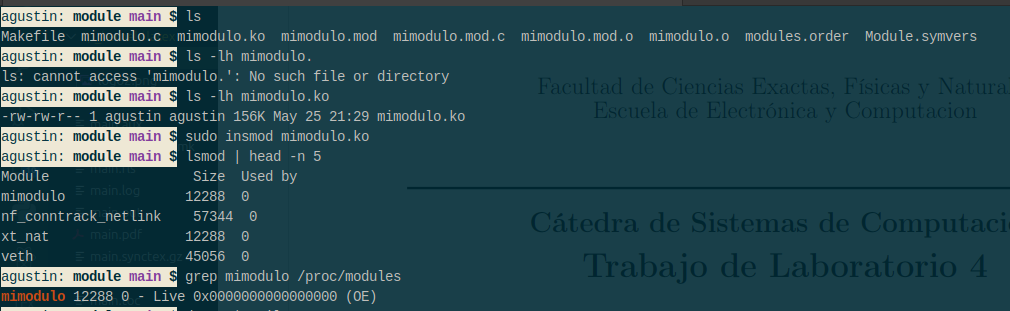
\includegraphics[width=0.8\linewidth]{images/paso1.png}
  \caption{Compilación y analisis del modulo.}
\end{figure}


\begin{figure}[h!]
  \centering
  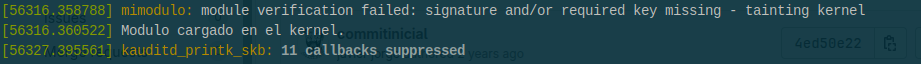
\includegraphics[width=0.8\linewidth]{images/kernellog.png}
  \caption{Log del kernel respecto al modulo propio.}
\end{figure}

\newpage

\section{Mejorar la seguridad del kernel: evitar modulos no firmados y mitigar rootkits}

Para fortalecer la seguridad del kernel es fundamental restringir la carga de modulos a aquellos que esten firmados y provenientes de fuentes confiables. A continuacion se enumeran acciones concretas respaldadas por la bibliografia consultada\footnote{Referencias: \emph{Linux Kernel Documentation: Kernel Lockdown}, \emph{Red Hat Secure Boot Guide}, \emph{The Art of Linux Kernel Design}.}:

\begin{enumerate}[label=\arabic*.]
  \item \textbf{Habilitar Secure Boot}: garantiza que el kernel y los modulos solo se carguen si estan firmados con claves de confianza (seccion~4).
  \item \textbf{Compilar el kernel con \texttt{CONFIG\_MODULE\_SIG\_FORCE=y}}: obliga a que cada modulo tenga firma valida; el kernel rechazara los no firmados.
  \item \textbf{Usar \texttt{module.sig\_enforce=1}} en la linea de comandos del kernel: equivalente en tiempo de arranque si el kernel ya se compilo con \texttt{CONFIG\_MODULE\_SIG}.
  \item \textbf{Implementar Lockdown Mode}: en kernels recientes (\texttt{CONFIG\_LOCKDOWN\_LSM}), opcionalmente activa restricciones adicionales que bloquean la manipulacion de memoria del kernel desde user space, incluso para \texttt{root}.
  \item \textbf{Activar SELinux/AppArmor perfiles estrictos}: reduce superficie de ataque para procesos potencialmente comprometidos que podrian intentar insertar modulos.
  \item \textbf{Deshabilitar \texttt{LOAD\_PIN\_ENFORCE}} (Lockdown PIN) solo si se requiere cargar modulos externos; de lo contrario, mantenerlo en enforcing.
  \item \textbf{Depurar modulos propios}: compilar con \texttt{-fstack\-protector\-strong}, \texttt{-D\_FORTIFY\_SOURCE=2}, habilitar CFI (\textit{Control Flow Integrity}) donde sea posible.
  \item \textbf{Monitorear firmas y blacklist}:
    \begin{itemize}[nosep]
      \item Revisar \texttt{/proc/sys/kernel/module\_sig\_enforce} (1 = obligatorio).
      \item Gestionar \texttt{.blacklist} del keyring para revocar claves comprometidas.
    \end{itemize}
  \item \textbf{Herramientas de deteccion de rootkits}: instalar y ejecutar periodicamente \texttt{rkhunter} y \texttt{chkrootkit}. Configurar alertas ante cambios en modulos del kernel o binarios criticos.
\end{enumerate}

Estas medidas, combinadas con un proceso de firmas propio (ver seccion de firma de modulos) y la generacion de paquetes reproducibles mediante herramientas como \texttt{checkinstall} o \texttt{dpkg-buildpackage}, minimizan el riesgo de rootkits que se basan en la insercion de modulos no autorizados.




\newpage
\section{Módulo anticheat.c: Monitoreo de acceso a archivos usando kprobe}

\subsection{Introducción y objetivo}

El archivo \texttt{anticheat.c} implementa un \textbf{módulo de kernel de Linux} diseñado para monitorear los intentos de acceso a un archivo específico en el sistema, simulando una funcionalidad básica de anti-cheat o protección. El objetivo es demostrar cómo los módulos de kernel pueden intervenir en operaciones sensibles y evidenciar la importancia de la seguridad al cargar módulos.

\subsection{¿Qué es \texttt{kprobe}?}

\texttt{kprobe} (kernel probe) es una interfaz del kernel de Linux que permite interceptar la ejecución de cualquier función interna del kernel, de forma dinámica y sin necesidad de recompilarlo. Al registrar un kprobe sobre una función, se puede ejecutar un ``handler'' (callback) personalizado cada vez que esa función es llamada.

En este contexto, kprobes se utiliza para \textbf{monitorear la apertura de archivos} mediante la interceptación de funciones como \texttt{do\_sys\_openat2} o \texttt{ksys\_openat}, que son responsables de manejar las llamadas \texttt{open()} y \texttt{openat()} en el kernel. Esta técnica es comúnmente empleada para debugging, profiling y tareas de monitoreo o seguridad.

\subsection{Descripción del funcionamiento}

El módulo \texttt{anticheat.c} registra un kprobe sobre la función interna del kernel encargada de abrir archivos. Cada vez que cualquier proceso intenta abrir un archivo, el handler del kprobe compara el nombre del archivo con una ruta específica (en este caso, \texttt{/tmp/trampa.txt}). Si coincide, el módulo imprime un mensaje de advertencia en el log del kernel, indicando el intento de acceso y el \texttt{PID} del proceso.

\begin{itemize}
    \item \textbf{No bloquea} el acceso: sólo lo detecta y lo registra para análisis.
    \item Es totalmente transparente para los programas de usuario.
    \item Demuestra el poder (y los riesgos) de los módulos para vigilancia y monitoreo a bajo nivel.
\end{itemize}
\newpage
\subsection{Código principal resumido}

\begin{verbatim}
/**
 * @file anticheat.c
 * @brief Módulo kernel: Monitorea acceso a archivo usando kprobe.
 * @author Tu Nombre
 */

#include <linux/module.h>
#include <linux/kernel.h>
#include <linux/kprobes.h>
#include <linux/uaccess.h>

#define FILE_MONITORED   "/tmp/trampa.txt"
#define PATH_LEN        128

static struct kprobe kp;

static int handler_pre(struct kprobe *p, struct pt_regs *regs)
{
    char filename[PATH_LEN] = {0};
#if defined(__x86_64__)
    char __user *user_filename = (char __user *)regs->si;
#elif defined(__aarch64__)
    char __user *user_filename = (char __user *)regs->regs[1];
#else
    #error "Arquitectura no soportada por este ejemplo"
#endif

    if (user_filename) {
        if (strncpy_from_user(filename, user_filename, PATH_LEN) > 0) {
            if (strcmp(filename, FILE_MONITORED) == 0) {
                printk(KERN_WARNING "[anticheat] Intento de abrir '%s' por PID %d (%s)\n",
                       filename, current->pid, current->comm);
            }
        }
    }
    return 0;
}

static int __init ac_init(void)
{
    kp.symbol_name = "do_sys_openat2";
    kp.pre_handler = handler_pre;
    register_kprobe(&kp);
    printk(KERN_INFO "[anticheat] Módulo cargado.\n");
    return 0;
}

static void __exit ac_exit(void)
{
    unregister_kprobe(&kp);
    printk(KERN_INFO "[anticheat] Módulo descargado.\n");
}

module_init(ac_init);
module_exit(ac_exit);

MODULE_LICENSE("GPL");
MODULE_AUTHOR("Tu Nombre");
MODULE_DESCRIPTION("Logger de intentos de apertura de archivo específico usando kprobe");
\end{verbatim}

\subsection{Funcionamiento y pruebas}

\begin{enumerate}
    \item \textbf{Compilación:} 
    \begin{verbatim}
    make
    \end{verbatim}
    \item \textbf{Carga del módulo:}
    \begin{verbatim}
    sudo insmod anticheat.ko
    \end{verbatim}
    \item \textbf{Prueba:} 
    Ejecutar cualquier comando que intente abrir el archivo monitoreado:
    \begin{verbatim}
    cat /tmp/trampa.txt
    \end{verbatim}
    \item \textbf{Ver logs del kernel:}
    \begin{verbatim}
    dmesg | tail
    \end{verbatim}
    Se verá una línea como:
    \begin{verbatim}
    [anticheat] Intento de abrir '/tmp/trampa.txt' por PID 12345 (cat)
    \end{verbatim}
    \item \textbf{Descarga del módulo:}
    \begin{verbatim}
    sudo rmmod anticheat
    \end{verbatim}
\end{enumerate}
\newpage
La siguiente imagen muestra el log del kernel sobre el intento de usar cat en trampa.txt

\begin{figure}[h!]
  \centering
  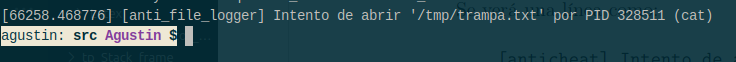
\includegraphics[width=0.8\linewidth]{images/dmesg.png}
  \caption{Log kernel por 'cat'}
\end{figure}


\end{document}
